% Created 2020-06-02 Tue 12:38
% Intended LaTeX compiler: pdflatex
\documentclass{article}
                                  \usepackage[nonatbib]{neurips_2020}
\usepackage[utf8]{inputenc}
\usepackage[T1]{fontenc}
\usepackage[table,svgnames]{xcolor}
\PassOptionsToPackage{hyphens}{url}\usepackage[hidelinks]{hyperref}
\usepackage{microtype}
\usepackage{graphicx}
\usepackage{amsmath}
\usepackage{amssymb}
\usepackage{multirow}
\usepackage{mathtools}
\usepackage{nicematrix}
\usepackage{cleveref}
\usepackage{txfonts}
\usepackage{bm}
\usepackage[backend=bibtex,natbib]{biblatex}
\renewcommand{\vec}[1]{\bm{#1}}
\newcommand{\Set}[1]{\mathcal{#1}}
\renewcommand{\Pr}{\text{P}}
\newcommand{\todo}[1]{{\color{red}TODO: #1}}
\addbibresource{./references.bib}
\author{Maximilian Nickel}
\date{}
\title{Latent Coupling for High-Resolution \\  COVID-19 Spread Forecasting}
\hypersetup{
 pdfauthor={Maximilian Nickel},
 pdftitle={Latent Coupling for High-Resolution \\  COVID-19 Spread Forecasting},
 pdfkeywords={},
 pdfsubject={},
 pdfcreator={Emacs 26.3 (Org mode 9.4)}, 
 pdflang={English}}
\begin{document}

\maketitle
\author{}


\begin{abstract}
Modeling the spread of COVID-19 at a high spatial and temporal resolution has
become a key task in the public health response to the disease. This poses
unique challenges due to the novelty of the disease, its unknown
characteristics, and substantial but varying interventions to reduce its spread.
To alleviate this issue, we propose a new method to disentangle the properties
of the underlying contagion process from its concrete realizations across
spatial entities. Our aim is to separate region-specific aspects -- such as
demographics, enacted policies, and testing methods -- from disease-inherent
aspects that influence its spread. This allows us to train high-resolution
models which jointly model the spread and are able to borrow strength across
regions. In our experiments, we demonstrate that our approach achieves
state-of-the-art performance in predicting the spread of the COVID-19 and
improves the robustness of forecasts.
\end{abstract}

\section{Introduction}
\label{sec:org3adcb67}
\begin{itemize}
\item Forecasting the spread the of COVID-19 is an important task in the public
health response to the disease. Not only important to understand the progress
of the disease, but also central to efficiently allocate scarce resources such
as ventilators, personal protective equipment, and ICU beds.
\item For resource allocation, it is especially important to do forecasts with a
high spatial and temporal resolution
\item Early detection of outbreaks
\item At the same time, forecasting COVID-19 poses unique challenges
\begin{itemize}
\item Novel disease with unknown characteristics
\item Very few data, especially at the beginning of the spread. However even
several months after the initial outbreak substantially less data than for other
infectious diseases like influence, measles etc.
\item Simultaneous spread in regions with very different properties
\begin{itemize}
\item demographics and population density
\item enacted policies
\item adherence to enacted policies
\item general mobility
\item geographic features such as temperature
\item testing and reporting
\end{itemize}
\end{itemize}
\item We build on prior work using autoregressive models designed for spatially and
temporally aggregated surveillance data of endemic-epidemic processes
\citep{held2005statistical,meyer2014powerlaw,meyer2016socialcontact}. Such
autoregressive models are, for instance, used to monitor infectious diseases
by public health agencies like Robert Koch Institute \citep{salmon2016surveillance}
\end{itemize}

\section{Method}
\label{sec:org51a8bb1}
\begin{itemize}
\item We assume we have a set of time series which are different realizations of the
the same underlying contagion process.
\item Let \(\Set{Y} = \{(y_i^1, \ldots, y_i^T)\}_{i=1}^M\) denote the observed
realizations and let \(\Set{Z} = \{(z_i^1, \ldots, z_i^T)\}_{i=1}^M\) denote the
underlying contagion process.
\item We want to disentangle different aspects in the model and couple the shared
aspects across regions
\item Hazard
In an SIR model, given \(y_t\) infected individuals at time \(t\), the hazard (or
force of infection) for a susceptible person at time \(t\) is given by
\[
  \lambda^\dagger_{t+1} = c(N) \frac{y_t}{N} p,
  \]
where \(c(N)\) denotes the unit rate of contacts that a susceptible person
experiences, \(y_t/N\) denotes the probability that a random contact is
infectious and
\(p\) denotes the probability of infection per contact.
\item Autoregressive models can be understood in a similar framework
\begin{equation*}
  \lambda
\end{equation*}
\item Autoregressive model of order \(p\)
\begin{equation}
  \text{AR}(p): y^{t+1} = \sum_{k=0}^p w_k y^{t-k} + \epsilon
\end{equation}
\item Our assumption is that the \emph{underlying} process is identical across sites,
i.e.,
\begin{equation}
  \forall i: z_i^{t+1} = \sum_{k=0}^p w_k z_i^{t-k} + \epsilon
\end{equation}
\item To disentangle aspects, we use a factorized representation
\begin{equation}
\beta_i^t w_k \approx \alpha_{ij }\beta_j^t w_k
\end{equation}

\begin{description}
\item[{\(\beta_i^t\)}] time-dependent scaling of the underlying process (e.g.,
through policies, social distancing etc.). Similar
\item[{\(\alpha_{ij}\)}] 
\end{description}
\end{itemize}

\subsection{Time Varying Process}
\label{sec:org55ef7a0}
\begin{equation*}
    y_{t+1} = \beta_t AR(p)
\end{equation*}

Many possible parameterizations for \(\beta_i^t\). For simplicty, we use a classic Elman RNN
where
\begin{align*}
    \beta_i^t & = \sigma(\vec{w}^\top \vec{z}_t)
    & \vec{z}_t & = \psi(W_z\vec{h}_t + \vec{b}_z) \\
    && \vec{h}_t & = \psi(W_h\vec{x} + U\vec{h}_{t-1} + \vec{b}_h)
\end{align*}

\subsection{Latent Coupling}
\label{sec:org5c315f5}

\subsubsection{Univariate Coupling}
\label{sec:org287edf9}
\begin{equation}
    y_i^{t+1} = \beta_i \sum_{k=0}^p w^k y_i^{t-k} + \epsilon
\end{equation}

\subsubsection{Multivariate Coupling}
\label{sec:orgf764c4f}
\begin{equation}
    y_i^{t+1} = \beta_i \sum_{k=0}^p \sum_{j=1}^m w^k \alpha_{ij} y_j^{t-k} + \epsilon
\end{equation}

Direct reqgularization of form
\begin{equation*}
    \sum_i\sum_j\sum_t\|\beta_i^t y_i^t - \alpha_{ij}\beta_i^t y_j^t\|^2
\end{equation*}
is problematic: runtime is \(O(M^2T)\). Moreover, not all pairs can be aligned.



\subsection{Maximum Likelihood Estimation}
\label{sec:orgc6d14df}
The popularity of the NB distribution is due largely to its ability to model
count data with varying degrees of overdispersion. The distribution is commonly
expressed in terms of the mean \(\mu\) and dispersion parameter \(\nu\) such that the
probability of observing a non-negative integer \(y\) is

\begin{equation*}
\Pr(Y = y) = \frac{\Gamma(y + \nu)}{y!\Gamma(\nu)}\left(\frac{\mu}{\mu +\nu}\right)^{y}\left(1 + \frac{\mu}{\nu}\right)^{-\nu}
\quad \mu > 0, \nu > 0
\end{equation*}

\begin{equation*}
    y^{t+1}_{i} \sim \text{NB}(\eta_i^{t}, \nu_i)
\end{equation*}

\begin{equation*}
    \min_\theta -\sum_{y} \log \Pr_\theta(Y = y)
\end{equation*}

\begin{minipage}{.335\linewidth}
\begin{center}
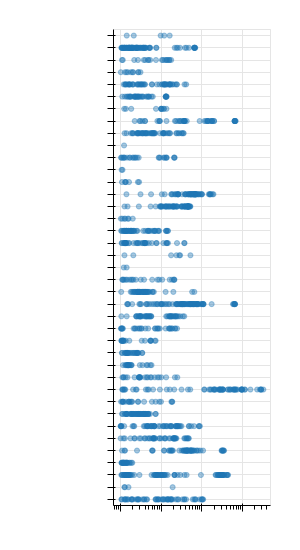
\includegraphics[width=\columnwidth]{img/overdispersion_states.png}
\end{center}
\end{minipage}
\begin{minipage}{.45\linewidth}
\begin{center}
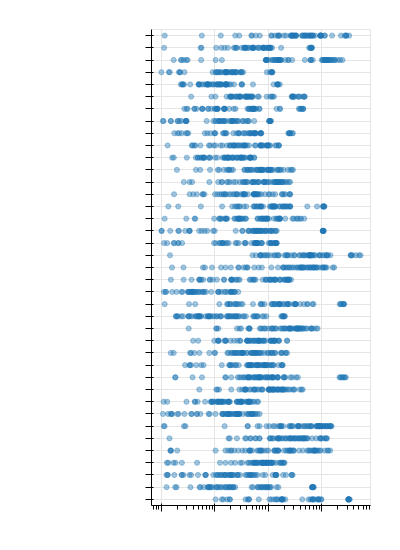
\includegraphics[width=\columnwidth]{img/overdispersion_counties.png}
\end{center}
\end{minipage}

\subsubsection{Training details}
\label{sec:org0c53443}
\begin{itemize}
\item We initialize the dispersion parameters to \(\log(nu_i) = 7\). This allows for
variance during the initial training and prevents the RNN from overfitting
\end{itemize}

\section{Related Work}
\label{sec:org4d03be1}
\cite{lloyd_smith2007negativebinomial}
\begin{itemize}
\item We are not regressing dependent variables onto counts. Instead we use latent
variables to disentangle and couple the different time series to infer the
structure of the underlying process.
\end{itemize}

\section{Experiments}
\label{sec:orgd50071c}
\subsection{Main Experiment}
\label{sec:org7a8df4c}
\begin{itemize}
\item Forecast Deaths and Confirmed Cases
\item Weekly backfill on US Nytimes data
\item Weekly backfill on Italy/Spain
\item Separate forecast horizons (allows us to also do CV on earlier days)
\begin{itemize}
\item 7 days
\item 14 days
\item 21 days
\end{itemize}
\item Baselines
\begin{itemize}
\item Standard AR model (univariate)
\item Standard AR model (multivariate)
\item S(E)IR
\item MHPs
\item Naive
\end{itemize}
\end{itemize}

**
\subsection{Ablation}
\label{sec:org1aae541}
\begin{itemize}
\item Univariate
\item Multivariate
\item Without Negative Binomial
\item Without Latent Beta
\item Without Coupling
\end{itemize}

\subsection{Analysis of Adjacency matrices}
\label{sec:orgbce42b4}
\begin{itemize}
\item coupled
\item uncoupled
\item l1/Granger regularization
\end{itemize}

\section{Conclusion}
\label{sec:org184985c}

\printbibliography
\end{document}
